\chapter{Algorítmos Meta-Heurísticos e Inteligência de Enxames}

As técnicas de Inteligência de Enxames (IE) estão inseridas dentro Computação Evolutiva, apesar de trazer uma metáfora diferente da evolução das espécies. Na IE, o comportamento biológico de seres vivos serve de inspiração o que torna as técnicas de otimização mais simples e fáceis de serem implementadas do que as técnicas evolucionárias.

Chan e Tiwari (2007) \cite{chan2007preface}, em seu livro “Swarm Intelligence: Focus on Ant and Particle Swarm Optimization”, expõem que a complexidade crescente dos problemas exigiu que os pesquisadores encontrassem o possível formas de facilitar a solução dos problemas. Segundo os autores, isso motivou os pesquisadores a compreender ideias da natureza e implantá-lo nas ciências da engenharia. Esse modo de pensar levou a surgimento de muitos algoritmos biologicamente inspirados que provaram ser eficientes em lidar com os problemas computacionalmente complexos com competência, tais como Algoritmo Genético (GA), Otimização de Colônia de Formigas (ACO), Otimização de Enxame de Partículas (PSO), etc.

Na IA, de acordo com Eberhart e Kennedy (2001) \cite{eberhart2001swarm}, o comportamento global do enxame é um efeito emergente das interações locais dos membros do enxame. De acordo com \cite{carmelo} as informações pessoais e sociais guardam semelhança com operadores de recombinação e de cruzamento, enquanto que a conservação de movimento da partícula atua como uma espécie de mutação direcional. Há diferenças, no entanto, sendo a maior delas o papel da seleção natural: enquanto que métodos evolutivos tem como parte essencial a morte dos indivíduos menos aptos, em um processo social os indivíduos são preservados durante a execução do algoritmo, de forma que o próprio indivíduo se adapta no decorrer do tempo.

Há uma série algoritmos de otimização de problemas que abordam diferentes grupos de seres vivos, desde pássaros a vagalumes para resolver problemas de otimização. Engelbrecht (2006) \cite{engelbrecht2006fundamentals} exemplifica alguns problemas resolvidos pela IE como aproximação de funções, agrupamento, otimização de estruturas mecânicas, resolução de sistemas de equações, otimização de roteamento em redes de telecomunicações, coloração de grafos, programação e resolução do problema de atribuição quadrática, dentro outros. Os problemas aqui tratados são conhecidos tecnicamente por NP-difícil. Portanto, técnicas computacionais mais apuradas são necessárias para resolver esses problemas.


Dentro da IE, há várias técnicas que abordam diferentes grupos de seres vivos desde pássaros a bactérias. Entretanto, este trabalho faz uso das seguintes abordagens: \textit{ Ant Colony Optimization} (ACO), \textit{Particle Swarm Optimization} (PSO) e \textit{Fish School Search} (FSS). O ACO, Otimização por Colônia de Formigas, tem a sociedade organizada das formigas como modelo para busca de alimentos através de rastros deixados pelas formigas. Já o PSO, Otimização por Enxame de Partículas, tem como inspiração os bandos de pássaro, tendo como a forma de voar em grupo na busca de alimento e mecanismo de interação social. Por fim, o FSS, Busca em Cardume de Peixes, tem no movimento do nado dos peixes a inspiração para proteção e busca de locais mais favoráveis para sobrevivência.

% ---
\section{ACO}
\label{sec-aco}
% ---

O ACO, desenvolvido por Dorigo e sua equipe em 1996 \cite{dorigo1996any}, inspirou-se no comportamento de colônias de formigas reais, em particular, por seu comportamento de forrageamento. Uma das principais ideias é a comunicação indireta entre os indivíduos de uma colônia de agentes, chamados de formigas, com base em uma analogia com trilhas de uma substância química, chamada feromônio, que as formigas reais utilizam para a comunicação. As trilhas (artificiais) de feromônio são um tipo de informação numérica distribuída que é modificada pelas formigas para refletir sua experiência acumulada ao resolver um problema particular.

Como descreve Mulati, Constantino e da Silva (2013) \cite{mulati2013otimizaccao}, foi descoberto que a comunicação entre as formigas que caminhavam pela trilha ocorria por meio de uma substância química, denominada feromônio, depositada por elas próprias. Enquanto as formigas caminham por uma trilha, inicialmente de forma aleatória, elas depositam uma certa quantidade de feromônio no solo. Assim, as próximas formigas tomam a decisão de seguir um caminho com probabilidade proporcional à quantidade feromônio depositada anteriormente. Ao decidir seguir um caminho com a presença da substância, ocorre então um reforço do caminho com o seu próprio feromônio. Este comportamento é denominado de auto-catalítico por ser um processo que reforça a si mesmo. O feromônio depositado tende a evaporar com o tempo, então quanto maior é a concentração de formigas passando pelo mesmo lugar, mais atrativo ele se torna para as próximas formigas. A Figura \ref{fig_aco} ilustra um experimento com formigas reais.

\begin{figure}[h]
	\caption{\label{fig_aco}Ilustração do experimento com formigas}
	\begin{center}
	    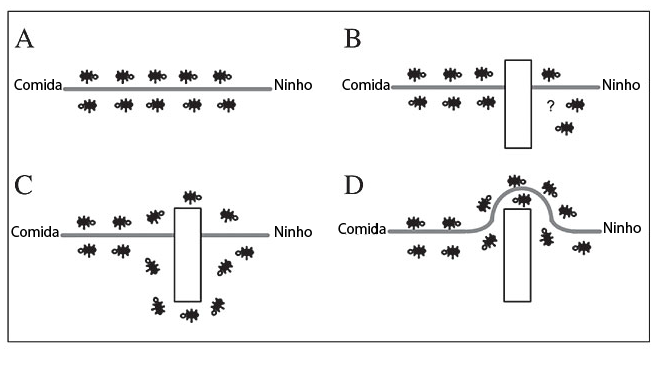
\includegraphics[scale=0.5]{imagens/aco-sample.png}
	\end{center}
	\legend{Fonte: Google Images}
\end{figure}


As formigas conseguem obter um bom caminho entre dois pontos. Na primeira decisão após a inserção do obstáculo, as quantidades de formigas a escolher o caminho mais curto e o caminho mais longo devem ser aproximadamente a mesma, de modo que elas escolhem o caminho com base no feromônio encontrado, sendo que as probabilidades de ambos os lados devem ter valores próximos um do outro. Porém, na segunda decisão, as formigas que percorreram o caminho mais curto já estão voltando, depositando ainda mais feromônio, enquanto as que foram pelo caminho mais longo ainda estão completando a primeira transição. Desta forma, as formigas tendem a seguir caminho mais curto.

De forma análoga, um indivíduo da colônia artificial constrói soluções candidatas, começando com uma solução vazia e, em seguida, adicionando componentes solução de forma iterativa até uma solução candidata completa ser gerada. Após a construção da solução estar completa, as formigas dão feedback das soluções que elas construíram depositando feromônio nos componentes da solução que elas usaram em sua solução. Tipicamente, os componentes da solução que fazem parte de melhores soluções ou são usados por muitas formigas receberão uma maior quantidade de feromônio. Portanto, provavelmente estes componentes serão usados pelas formigas em iterações futuras do algoritmo. Para evitar que a busca fique estagnada, geralmente antes das trilhas de feromônio serem reforçadas, todas as trilhas de feromônio são diminuídas por um fator $\rho$.

Em geral, todos os algoritmos ACO para combinação combinatória estática seguem um esquema algorítmico específico mostrado no Pseudocódigo \ref{alg:aco}. Após a inicialização do trilhas de feromônio e alguns parâmetros, um loop principal é repetido até uma condição de término - que pode ser um certo número de construções de soluções ou um determinado limite de tempo de CPU - é cumprido. No loop essencial, primeiro, as formigas constroem soluções viáveis, então as soluções geradas podem ser melhoradas pela aplicação busca local e, finalmente, as trilhas de feromônios são atualizados.

\begin{algorithm}
	\caption{Ant Colony Optimisation}\label{alg:aco}
	\begin{algorithmic}[1]
		\small
        \State{Configurar parametros, inicializar as trilhas de feromônio}
        \
		\State{Enquanto o critério de parada não é satisfeito:}
        \State{Para cada uma das formgias(em parelelo):}
        \State{Construi soluções}
        \State{Aplique Busca Local (opcional)}
        \State{Atualize as trilhas}
	\end{algorithmic}
\end{algorithm}

% ---
\section{ACS}
\label{sec-acs}
% ---

O algoritmo \textit{Ant Colony System}, ou Sistema de Colônia de Formigas, é  uma abordagem derivada da Otimização de Colônia de Formigas (ACO) também desenvolvida por Dorigo et al. (2006) \cite{dorigo2008particle}. O ACS difere do ACO em três pontos principais: utiliza uma Regra de Transação de Estado (RTE) mais agressiva; a Regra de Atualização do Feromônio (RAF) determina a evaporação e o depósito do feromônio nas arestas que fazem parte da melhor solução corrente, isto é, a melhor solução já encontrada até o momento em uma iteração; e a cada utilização de uma aresta, uma quantidade pré-definida de feromônio é removida. A proposta de remover o feromônio no ACS serve para aumentar a diversificação das soluções.

As formigas inicialmente vagam aleatoriamente em torno de seu ambiente. Quando o alimento é localizado a formiga começa a disseminar o feromônio no ambiente. A adição do feromônio pelo caminho no decorrer de inúmeras viagens. Entretanto, os feromônios se deterioram no ambiente. Cada formiga deposita uma quantidade de feromônio que diminui de acordo com seu ranque.

Através de elitismo, faz uso de intensificação, escolhendo com maior probabilidade cidades promissoras. Assim, apenas a formiga com a melhor solução corrente (\textit{best-so-far}) deposita feromônio.

A RAF do ACS define que a atualização de feromônio ocorre em dois momentos: uma atualização global, ao final de cada iteração do algoritmo; e uma atualização local, logo depois que uma formiga se move de uma cidade a outra, ou seja, inclui mais uma aresta na sua rota.

% ---
\section{TACO}
\label{sec-taco}
% ---

A Otimização de Colônia de Formigas (TACO), proposta por Vallivaara (2008) \cite{vallivaara2008team}, é baseada no ACS para resolver instâncias de MTSP. Essa generalização básica é feita substituindo as $N$ formigas ACS, que constroem soluções para o TSP, com $N$ equipes de $m$ membros. Uma equipe de formigas representa um vendedor na construção da solução MTSP e cada equipe tem sua lista de tabu.

Todas as formigas de cada equipe são colocadas no depósito no início da construção da rota. Para distribuir a carga de trabalho, uma formiga com a rota parcial mais curta escolhe sua próxima cidade j, em qualquer momento do processo de construção, de acordo com a equação da Regra de Estado de Transição (RET), conforme mostrado em \ref{eq:taco-ret}.

\begin{equation} \label{eq:taco-ret} 
    j = \Bigg\{
        \begin{tabular}{ll}
        argmax\(_{l \in J_k} \{\tau_{il}[\eta_{il}]^\beta\}\), & if $q \leq q_0$ \\
        J, & otherwise;
        \end{tabular}
\end{equation}

Depois de escolher a cidade seguinte, verifica-se se outra formiga poderia adicionar a cidade escolhida à sua rota e acabar com uma melhor duração total da rota. Se assim for, essa formiga pode fazer seu primeiro movimento não escolhendo $j$. Esse ponto de verificação evita que o algoritmo force soluções não ideais.

TACO tem vários parâmetros que são responsáveis pelo seu comportamento durante a construção de soluções. A probabilidade inicial q0 determina se a inicialização das formigas tem apenas escolhas determinísticas ou aleatórias $(0 < q_0 <1)$. Os parâmetros de feromônio $\alpha$ e $\beta$ definem o peso da trilha de feromônio e a visibilidade, respectivamente, na escolha do próximo nó pela formiga. O parâmetro $\xi$ controla a persistência do feromônio quando a Regra de Atualização de Feromônio (RAF) ocorre localmente, logo após uma formiga se mover de uma cidade para outra, ou seja, inclui mais uma borda em sua rota. Da mesma forma, $\rho$ regula a persistência de feromônios para RAF global, ou seja, no final de cada ciclo do algoritmo.

Finalmente, o algoritmo usa uma abordagem de pesquisa local para melhorar as soluções construídas. A pesquisa local opt-2 altera quaisquer duas arestas de uma solução e verifica se ela obtém alguma melhoria. O procedimento opt-2 é aplicado a todas as soluções construídas.

% ---
\section{PSO}
\label{sec-pso}
% ---

Kennedy e Eberhart (1999) \cite{kennedy1999particle} propuseram o método \textit{Partition Swarm Optimization} (PSO) baseado no revoada das aves. O PSO é adequado para a otimização de variáveis contínuas em um espaço de busca de alta dimensão e apresenta alta precisão. Ele realiza a pesquisa por meio de um enxame de partículas por meio de um processo de iteração.

% \begin{algorithm}
% 	\caption{Particle Swarm Optimization}\label{alg:pso}
% 	\begin{algorithmic}[1]
% 		\small
% 		\State{Inicializar a posição \(x_i\), a velocidade \(v_i\) e a melhor posição pessoal \(P_{best}\) das \(N\) partículas}
%         \State{Enquanto o critério de parada não é satisfeito faça}
%         \State{Para \(j = 1\) até \(N\) faça:}
%         \State{\(G_{best}\) = }
%         \State{Análise dos resultados via gráficos e mapas de calor}
% 	\end{algorithmic}
% \end{algorithm}

Cada partícula se move em direção a sua melhor posição ($P_{best}$) anterior e a melhor posição global ($G_{best}$) no enxame para alcançar a solução ótima, como mostrado na Equação \ref{eq:pso-movement}.

\begin{equation} \label{eq:pso-movement}
    _{i(t+1)} = x_{i(t)} + v_{i(t)}
\end{equation}

A solução representa a posição da partícula no espaço de busca, um vetor $x_i$. Para cada etapa, as partículas têm suas posições de acordo com seu vetor de velocidade $v_i$, como mostrado na Equação \ref{eq:pso-speed}.

\begin{equation} \label{eq:pso-speed}
    v_j = \omega v_j + c_1 r_1(P_{best} - x_j) + c_2 r_2(G_{best} - x_j)
\end{equation} 

A velocidade de fixação, um limite superior para o parâmetro de velocidade evita que as partículas voem para fora do espaço de busca. Da mesma forma, a estratégia do "coeficiente de constrição", proposta por Clerc e Kennedy (2008) \cite{clerc2002particle}, constrói as velocidades através da análise dinâmica de enxames.

A inércia, mostrada na primeira parte da Equação \ref{eq:pso-clerc-speed}, representa a velocidade anterior, que fornece o momento necessário para as partículas percorrerem o espaço de busca.

\begin{equation} \label{eq:pso-clerc-speed}
    v_{ij}(t+1) = \chi[v_{ij}(t+1) + \varphi_1(v_{ij}(t) - x_{ij}(t)) + \varphi_2(\hat{y}_{ij}(t) - x_{ij}(t))]
\end{equation}

Por outro lado, o componente cognitivo, a Equação \ref{eq:pso-clerc}, determina o movimento individual de cada partícula. Ele incentiva as partículas a se moverem em direção às suas melhores posições atuais. 

\begin{equation} \label{eq:pso-clerc}
    \chi = \frac{2}{4 - \varphi - \sqrt{\varphi^2 - 4\varphi}}
\end{equation}

A último a Equação \ref{eq:pso-clerc-coefficient}, o componente "social", implica o efeito colaborativo das partículas para encontrar a solução global ótima.

\begin{equation} \label{eq:pso-clerc-coefficient}
    \varphi = C_1 + C_2, \varphi_1 = c_1, \varphi_2 = c_2
\end{equation}

% ---
\section{FSS}
\label{sec-fss}
% ---

Bastos-Filho et al. (2008) \cite{bastos2008novel} desenvolveu um algoritmo de busca de base populacional inspirado no comportamento de natação de peixes, que se expande e se contrai enquanto procura comida. O algoritmo \textit{Fish School Search} (FSS) considera os movimentos individuais e coletivos dos peixes. Esse algoritmo de otimização não apresenta a mesma capacidade de exploração do PSO, mas tem a capacidade de encontrar boas soluções em um espaço de pesquisa com muitos mínimos locais.

Cada peixe, em localização $n$-dimensional, representa uma solução viável para o problema. Seu sucesso é medido pelo seu peso, uma conta cumulativa do sucesso da busca por cada peixe na escola. Os peixes não apenas armazenam informações sobre seu peso, mas também se posicionam no espaço de busca.

O FSS consiste em operadores de movimentação e alimentação. No movimento individual, cada peixe se desloca aleatoriamente em direção a uma posição em sua vizinhança à procura de regiões promissoras. Este componente é calculado usando a Equação \ref{eq:fss-movement}.

\begin{equation} \label{eq:fss-movement}
    n_{ij} = x_{ij(t-1)} + step_{ind} \times random[-1,1]
\end{equation}

Depois de se mudar para novas posições, todos os peixes têm seus pesos atualizados de acordo com a Equação \ref{eq:fss-feeding}. A atualização de peso é determinada pelo sucesso do movimento individual, que é calculado através da adequação das posições atual e nova.

\begin{equation} \label{eq:fss-feeding}
    W_{i(t)} = W_{i(t-1)} + \frac{\Delta f_{i(t)}}{max[\Delta f_{i(t)}]}
\end{equation}

Depois de alimentar todos os peixes, ocorre o movimento coletivo-instintivo. Todos os peixes se movem em direção a um vetor de influência, como mostrado nas Equações \ref{eq:fss-fitness} e \ref{eq:fss-newmove}. Os peixes que melhoraram sua aptidão na iteração atual e geram esse vetor.

\begin{equation} \label{eq:fss-fitness}
    m_{j(t)} = \frac{\sum_{}^{} N_i = x_{ij(t)} \times W_{ij(t)}}{\sum_{}^{} N_i = W_{ij(t)}}
\end{equation}

\begin{equation} \label{eq:fss-newmove}
    x_{ij(t)} = x_{ij(t)} + m_{j(t)}
\end{equation}

No final da iteração atual, o cardume se contrai ou se expande de acordo com o operador do movimento volitivo-coletivo. A contração da escola resulta em uma busca de exploração, enquanto sua expansão faz com que a escola explore a área de busca, evitando os mínimos locais. Assim, o operador volitivo calcula o baricentro da escola como mostrado na Equação \ref{eq:fss-barycentre} e atualiza o seu movimento, de acordo com a Equação \ref{eq:moveagain}. Este último operador fornece ao FSS a capacidade de auto-ajustar a granularidade da pesquisa ao longo do processo de otimização.

\begin{equation} \label{eq:fss-barycentre}
    B_j = \frac{\sum_{}^{} x_{ij(t)W_{ij(t)}}}{\sum_{}^{} W_{ij(t)}}
\end{equation}

\begin{equation} \label{eq:moveagain}
    x_{ij(t)} = x_{ij(t)} \pm step_{vol}\frac{x_{ij(t) - B_j}}{dist(x_{ij(t)}, B_j)}
\end{equation}


% ---
\section{MOFSS}
\label{sec-mofss}
% ---

A Busca Multi-Objetiva da Escola de Peixes (MOFSS) é uma generalização FSS que lida com problemas com múltiplas restrições objetivas. Ele usa um Arquivo Externo (EA) para armazenar as melhores soluções não dominadas encontradas durante o processo de busca. As soluções no EA são usadas para guiar os movimentos dos peixes no espaço de busca. O método \textit{Crowding Distance} trunca o EA para lidar com seu limite de tamanho. O MOFSS difere do FSS nos operadores de seleção de recursos que são adaptados para resolver problemas multi-objetivos.

No movimento individual, o peixe sempre se move em direção a novas posições, mesmo que sejam piores que as anteriores ou as posições sejam indiferentes, considerando o critério de dominância. Soluções no EA levam os movimentos individuais. Para cada peixe, um guia é selecionado usando o operador de seleção de líder. A seleção é executada por um torneio que seleciona dois peixes e executa uma seleção aleatória para retornar um guia.

O movimento volitivo multi-objetivo leva o conjunto de soluções não dominadas da EA como pontos de referência para contratar ou expandir a escola, enquanto o FSS usa o baricentro escolar para determinar esses pontos. Cada peixe da escola seleciona um líder, usando o operador de seleção de líderes, e se move em direção a ele. Assim, os peixes tendem a se mover para as soluções não dominadas.

Finalmente, o operador de turbulência ocorre para evitar que o enxame fique preso nos mínimos locais. O operador cria novas posições vizinhas que são avaliadas em cada iteração. Se as novas posições forem soluções não dominadas, elas serão incluídas no EA.
